\chapter{Frameworks and Models for Stock Price Prediction}

\section{Overview of Proposed Architectures}
This chapter presents the various architectures and frameworks explored for stock price prediction, from initial experiments during the summer internship to advanced hybrid and feature-rich frameworks developed later. The focus is on improving prediction accuracy, addressing issues like lag, and incorporating domain-specific features. A systematic approach to model building, including feature engineering and model integration, is discussed.

\section{Hybrid LSTM-RLS Architecture}

\subsection{Workflow and Design}
The Hybrid LSTM-RLS Architecture was the first model developed during my summer internship. It combines the strengths of LSTM for capturing sequential dependencies and Recursive Least Squares (RLS) for refining predictions. Figure~\ref{fig:summerarch} illustrates the architecture, highlighting the key components and their interactions.

\begin{figure}[h!]
    \centering
    \includegraphics[width=0.8\textwidth]{Images/SummerInternArchitecture.pdf} % Adjust width as needed
    \caption{Hybrid LSTM-RLS Architecture}
    \label{fig:summerarch}
\end{figure}

The workflow for this architecture is as follows:
\begin{enumerate}
    \item \textbf{Install and load necessary libraries:} Libraries such as TensorFlow, NumPy, yfinance, and scikit-learn were installed and imported.
    \item \textbf{Load stock data using yfinance API:} Historical stock price data was fetched using the yfinance API.
    \item \textbf{Data preprocessing:} The data was normalized, missing values were handled, and it was split into training and testing sets.
    \item \textbf{Create sequences:} Price sequences of fixed length were created as input to the LSTM model.
    \item \textbf{Train the LSTM model:} The LSTM model was trained to predict the next stock price based on these sequences.
    \item \textbf{LSTM predictions passed to RLS model:} Scalar predictions from the LSTM model were passed to the RLS model.
    \item \textbf{RLS model provides final prediction:} The RLS model used the LSTM predictions to produce refined stock price predictions.
\end{enumerate}

\section{Enhanced Hybrid LSTM-RLS Architecture}

To address issues such as dimension mismatches and long training times in the original architecture, several enhancements were implemented during Semester 3. These refinements simplified the process and improved predictive accuracy.

Figure~\ref{fig:Refinedarch} illustrates the improved workflow. The modifications made the architecture more efficient and straightforward for stock price forecasting.

\subsection{Architecture Workflow}

\begin{figure}[htbp]
    \centering
    \includegraphics[width=0.8\textwidth]{Images/RefinedArchitecture.pdf} % Replace with the actual image file
    \caption{Enhanced Hybrid LSTM-RLS Architecture}
    \label{fig:Refinedarch}
\end{figure}

The architecture process involves the following steps:

\begin{enumerate}
    \item \textbf{Install and import necessary libraries:}
    \begin{itemize}
        \item Libraries such as \texttt{yfinance}, \texttt{tensorflow}, \texttt{scikit-learn}, and others were imported.
    \end{itemize}
    
    \item \textbf{Import Nifty 50 daily close price data:}
    \begin{itemize}
        \item Closing prices of the Nifty 50 index for the last 12 years were fetched daily using the \texttt{yfinance} API.
    \end{itemize}
    
    \item \textbf{Normalize the data:}
    \begin{itemize}
        \item Data was normalized and scaled to a range of 0 to 1 using \texttt{MinMaxScaler}.
    \end{itemize}
    
    \item \textbf{Sequence creation for LSTM:}
    \begin{itemize}
        \item Sequences of historical stock prices were created as inputs for training the LSTM model.
    \end{itemize}
    
    \item \textbf{Split dataset into training and testing set}
    \begin{itemize}
        \item The sequences were divided into training (80\%) and testing (20\%) sets to evaluate model performance.
    \end{itemize}
    
    \item \textbf{Training of the LSTM model:}
    \begin{itemize}
        \item The LSTM model was trained on the 80\% training data over several epochs to predict stock prices.
    \end{itemize}
    
    \item \textbf{Input Sequences creation for RLS:}
    \begin{itemize}
        \item Predictions from the LSTM model is used to prepare input sequences for the RLS model.
    \end{itemize}
    
    \item \textbf{Forecast Stock Prices with RLS:}
    \begin{itemize}
        \item The RLS model processed the LSTM predictions as inputs, producing the final stock price forecasts.
    \end{itemize}
    
\end{enumerate}

\subsection{Developing Input Sequences for RLS}

Figure~\ref{fig:inputseq} provides a detailed view of the sequence development process for the RLS model based on LSTM predictions.

\begin{figure}[htbp]
    \centering
    \includegraphics[width=0.8\textwidth]{Images/RLSInputCreation.pdf} % Replace with the actual image file
    \caption{Input Sequence Formation for RLS}
    \label{fig:inputseq}
\end{figure}

The following steps outline the process:

\begin{enumerate}
    \item \textbf{Original Sequence for LSTM:}
    \begin{itemize}
        \item The original sequence of stock prices served as the input for training the LSTM model.
        \item For example, a sequence ranging from index 0 to 49 was selected.
    \end{itemize}
    
    \item \textbf{Training the LSTM Model:}
    \begin{itemize}
        \item The LSTM model was trained on the input sequence.
        \item Upon training, the model predicted the 50th value based on the prior 49 values.
    \end{itemize}
    
    \item \textbf{Shifting the Sequence for RLS Input:}
    \begin{itemize}
        \item The sequence was shifted by one step to generate input for the RLS model.
        \item For instance, the updated sequence started at index 1 and extended to index 50, incorporating the LSTM prediction for the 50th point.
    \end{itemize}
    
    \item \textbf{Final Input for RLS Model:}
    \begin{itemize}
        \item The shifted sequence (from index 1 to 50) was provided as input to the RLS model.
        \item The RLS model used this sequence to produce the final stock price prediction.
    \end{itemize}
\end{enumerate}

This sliding window approach facilitated seamless integration between the LSTM and RLS models, ensuring improved accuracy and efficient stock price forecasting.

\subsection{Multi-Feature Hybrid LSTM-RLS Implementation}

In the \textbf{Hybrid LSTM-RLS architecture with a multi-feature dataset}, the dataset was utilized in its preprocessed form, eliminating the need for additional preprocessing steps. The overall workflow of the implementation is illustrated in \textbf{Figure~\ref{fig:HybridLSTM_RLS_M}}.

\begin{figure}[h!]
    \centering
    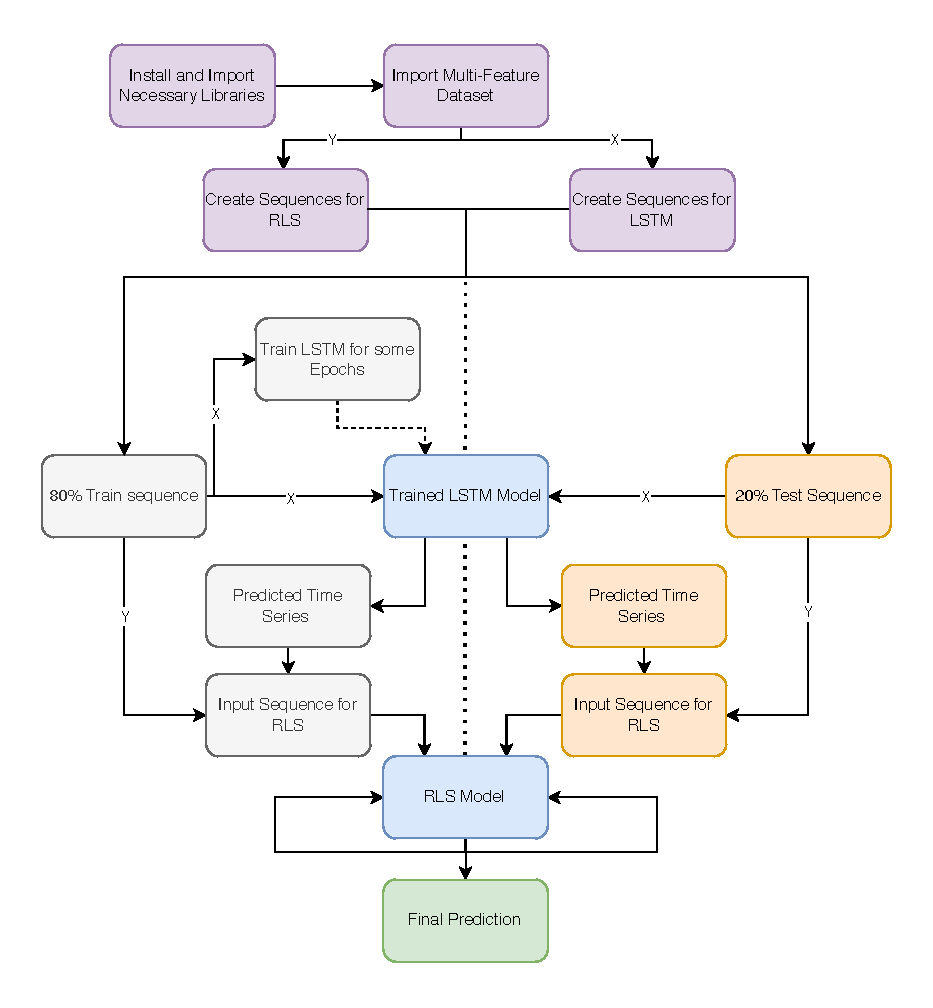
\includegraphics[width=0.8\textwidth]{Images/HybridLSTM_RLS_M.pdf}
    \caption{Flow diagram of Multi-Feature Hybrid LSTM-RLS implementation.}
    \label{fig:HybridLSTM_RLS_M}
\end{figure}

The LSTM model was trained following the standard sequence-based approach, where multi-feature input sequences were constructed and used for training.

\subsubsection{Key Modification: RLS Input Sequence Construction}

A significant deviation from the previous approach was the method used to construct input sequences for the \textbf{Recursive Least Squares (RLS) model}. As illustrated in \textbf{Figure~\ref{fig:RLS_Input_M}}, the input sequence creation for RLS followed a structured pipeline:

\begin{figure}[h!]
    \centering
    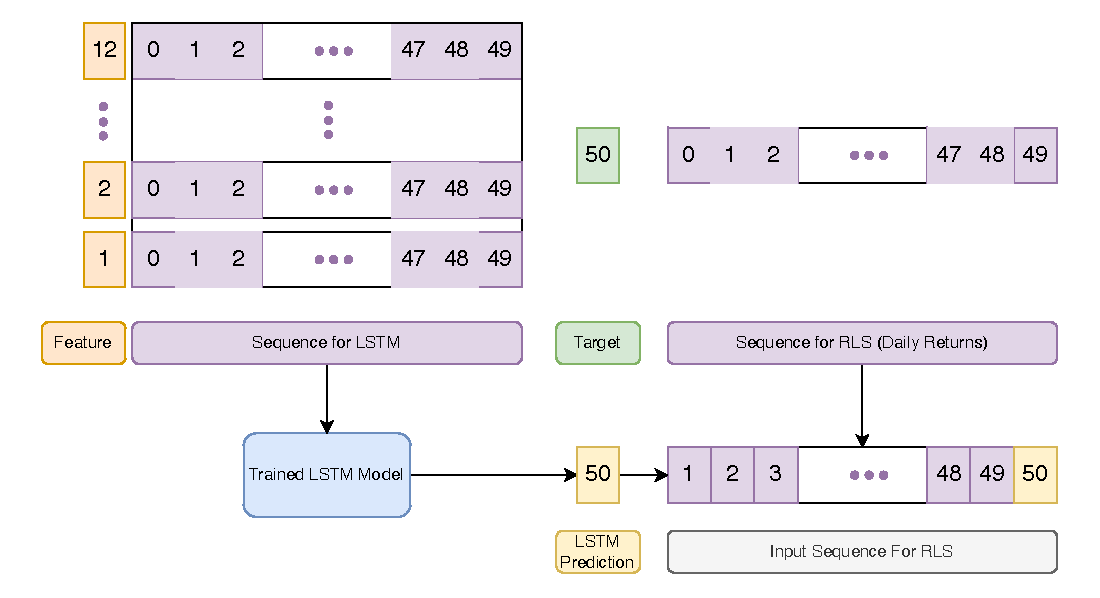
\includegraphics[width=0.8\textwidth]{Images/RLS_Input_M.pdf}
    \caption{RLS input sequence construction using LSTM outputs.}
    \label{fig:RLS_Input_M}
\end{figure}

\begin{itemize}
    \item Instead of deriving the RLS input sequences from the \textbf{LSTM input sequence}, the sequences were generated using \textbf{returns and close prices}.  
    \item The LSTM model was trained on sequences created from the \textbf{multi-feature input} (\textbf{X}). Once trained, the predicted values from LSTM were appended to the sequences constructed from \textbf{daily returns} (\textbf{Y}), ensuring that the RLS model receives inputs of the same nature as its output, thus allowing effective prediction in an online setting.
    \item Two separate training strategies were employed:  
    \begin{itemize}
        \item \textbf{Predicting Returns}: The model was trained to forecast stock returns, leveraging the structured relationship between past returns and future movements.  
        \item \textbf{Predicting Close Prices}: The model was also trained using close prices to evaluate its performance in direct price prediction.
    \end{itemize}
\end{itemize}

\subsubsection{Impact of this Approach}

\begin{itemize}
    \item \textbf{Alternative Feature Representation}: By constructing input sequences from returns and close prices, the model captured different aspects of market behavior.  
    \item \textbf{Comparative Performance Analysis}: Training for both returns and close prices allowed an in-depth evaluation of prediction effectiveness under different target variable choices.  
    \item \textbf{Flexible RLS Adaptation}: The RLS model benefited from this new input structure, enabling it to adjust dynamically to either return-based or price-based forecasts.  
\end{itemize}

This modification provided insights into how input sequence construction affects the overall model accuracy and adaptability, further refining the \textbf{Hybrid LSTM-RLS architecture}.

\section{Dual Network Solution (DNS) Architecture}
\subsection{Design and Integration}
The Dual Network Solution (DNS) architecture addresses the one-time-step lag observed in the previous models. Figure~\ref{fig:DNSArch} shows the DNS architecture, which involves two networks: one trained on trends and the other on actual data.

\begin{figure}[h!]
    \centering
    \includegraphics[width=0.8\textwidth]{Images/DNSArchitecture.pdf} % Adjust width as needed
    \caption{DNS Architecture}
    \label{fig:DNSArch}
\end{figure}

Steps include:
\begin{enumerate}
    \item \textbf{Trend extraction:} Network 1 is trained to predict trends using slope differences or moving averages.
    \item \textbf{Prediction refinement:} Network 2 uses the output of Network 1 to generate lag-free predictions.
\end{enumerate}

\section{Advanced Data Preprocessing for Enhanced Model Performance}
\subsection{Challenges in Scaling and Activation}
During the development of the stock price prediction models, challenges arose when scaling the data using traditional normalization techniques such as MinMaxScaler. This approach limits the range of predictions to the maximum value observed during training, potentially capping future predictions. To address this issue, an alternative preprocessing technique was introduced, which involves:
\begin{itemize}
    \item \textbf{Log Transformation:} Applying a logarithmic transformation to the close price values to reduce large variations and stabilize the data.
    \item \textbf{Standardization:} Standardizing the log-transformed values to ensure that the data is centered and scaled, allowing it to be processed effectively by the model.
\end{itemize}

After preprocessing, the resulting data ranged approximately between $-2$ and $2$. To handle this range, the \texttt{tanh} activation function was selected for its natural prediction range of $[-1, 1]$. However, to ensure flexibility in predictions beyond this range:
\begin{itemize}
    \item A multiplier of $2.5$ was applied after the \texttt{tanh} activation function. This adjustment extended the prediction range to $[-2.5, 2.5]$, providing additional room for extreme values without capping predictions.
\end{itemize}

Figure~\ref{fig:distribution_plot} shows the distribution plot of the raw close values, log-transformed close values, and scaled log-transformed values. This plot depicts how the preprocessing steps have allowed the data to fall in a range that the activation function can handle effectively.

\begin{figure}[h]
    \centering
    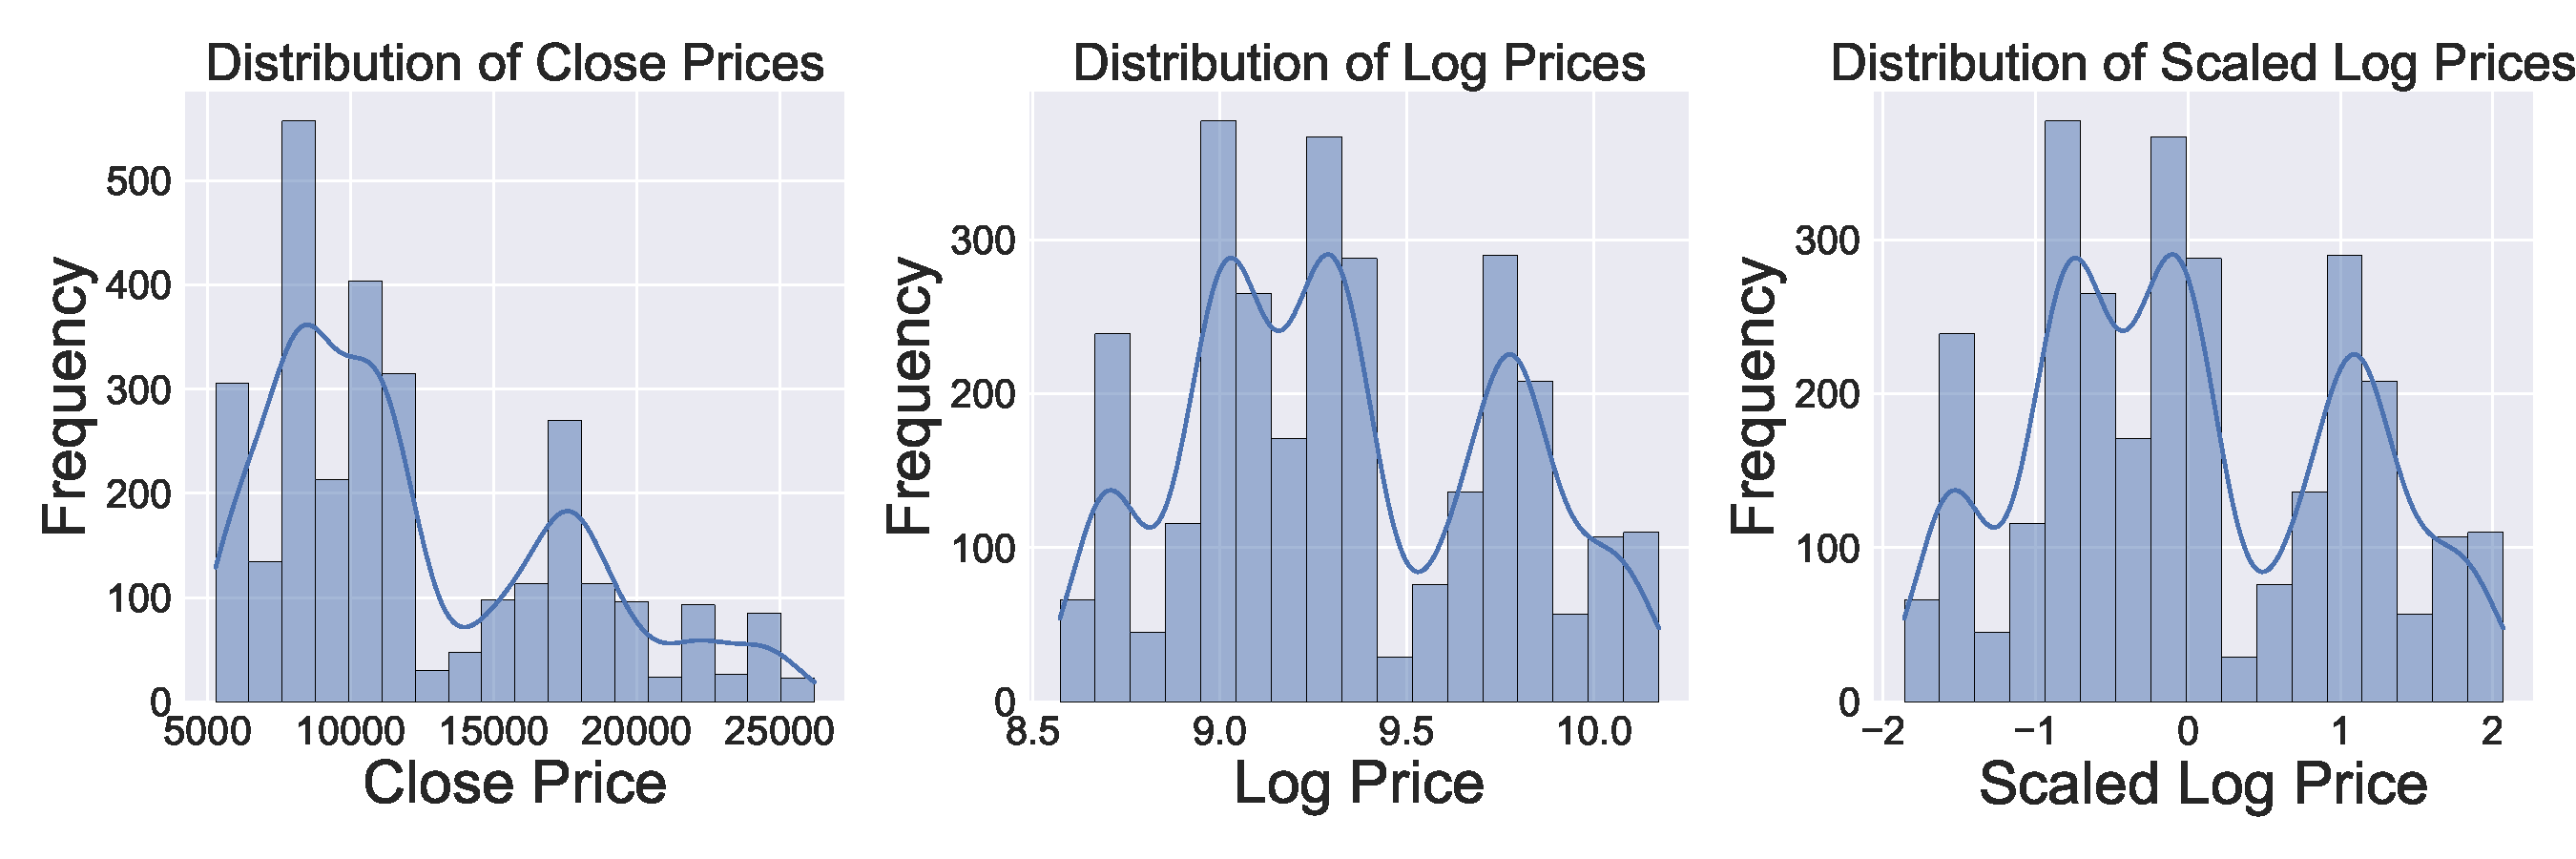
\includegraphics[width=\textwidth]{Images/distribution_plot.pdf}
    \caption{Distribution plot of raw close values, log-transformed close values, and scaled log-transformed close values.}
    \label{fig:distribution_plot}
\end{figure}

\subsection{Application in DNS Architecture}
This preprocessing technique, as explained in Section 3.5.1 was used in the concept of the Dual Network Solution Architecture. Using log transformation, standardization, and modified range of activation functions,
the DNS model represents both linear and nonlinear parts of
stock price movements.

This preprocess step was crucial in enhancing the prediction accuracy of the model.
racy of the DNS architecture, so that it could support a greater number of values
While the predictions of strength were retained, the changes had provided the basis for
groundwork for subsequent enhancements in model design and integration.


% \section{ARIMA-LSTM Residual Integration Framework}
% \subsection{Justification for ARIMA-LSTM Hybridization}
% This framework combines ARIMA's ability to model linear patterns with LSTM's strength in capturing non-linear relationships. The final prediction is obtained by integrating outputs from both models. Key components include:
% \begin{itemize}
%     \item \textbf{ARIMA model for linear trends:} ARIMA captures the linear component of stock prices.
%     \item \textbf{LSTM model for residuals:} LSTM models the non-linear residuals.
%     \item \textbf{Final integration:} Predictions from both models are combined for improved accuracy.
% \end{itemize}

\section{ARIMAX-LSTM Residual Integration Framework}
\subsection{ARIMAX-LSTM Hybridization}

The initial approach involved integrating the capability of ARIMA to model linear patterns and LSTM's strength in capturing non-linear relationships. However, due to suboptimal performance, the ARIMA model was replaced with ARIMAX for handling the linear component while LSTM continued to process residuals. The final prediction was obtained by integrating the outputs of these two models. The revised framework consists of:

\begin{itemize}
    \item \textbf{ARIMAX model for linear trends:} Unlike ARIMA, ARIMAX incorporates external features alongside past values to better capture the linear component of stock prices.
    \item \textbf{LSTM model for residuals:} LSTM models the remaining non-linear residuals after ARIMAX processing.
    \item \textbf{Final integration:} Predictions from both models are combined to enhance accuracy.
\end{itemize}

\subsection{Challenges and Model Refinement}

Initially, the ARIMA-LSTM hybrid model was tested; however, its performance was unsatisfactory. The residuals did not capture sufficient differences between the original close price values and ARIMA’s linear predictions, leading to subpar results. 

To address this issue:
\begin{itemize}
    \item The \textbf{ARIMA model was replaced with ARIMAX}, incorporating external variables to improve the modeling of linear relationships.
    \item The \textbf{LSTM model remained responsible for capturing non-linear residuals}.
    \item The integration of \textbf{ARIMAX and LSTM} was evaluated to determine if this modification led to improved performance.
\end{itemize}

This refined framework aimed to leverage ARIMAX's enhanced linear modeling alongside LSTM's capacity for non-linearity, ultimately improving the predictive capability of the model.

\subsection{Applying RLS to Residuals Framework Output}

In the \textbf{ARIMAX-LSTM-RLS model}, after predicting returns using the \textbf{ARIMA-LSTM Residual Integration Framework}, the next step involved incorporating \textbf{Recursive Least Squares (RLS)} to refine the final predictions.

\subsubsection{RLS Input Sequence Construction}

To enhance the prediction accuracy, input sequences for RLS were constructed as follows:
\begin{itemize}
    \item The predicted returns obtained from the \textbf{residuals architecture} were used to generate input sequences for RLS.
    \item RLS was then applied to these sequences, providing the \textbf{final predicted returns output}.
\end{itemize}

\subsubsection{Impact of RLS on the Residuals Architecture}

\begin{itemize}
    \item \textbf{Sequential Refinement}: By feeding the residuals architecture's output into RLS, the model aimed to further refine the predictions.
    \item \textbf{Performance Evaluation}: The final output from RLS was analyzed to determine whether this additional step improved the overall prediction accuracy.
\end{itemize}

This integration of RLS with the residuals architecture provided valuable insights into whether the additional layer of processing contributed to enhanced model performance.

% \section{Training Method for Multi-Feature LSTM Forecasting Framework}

% \subsection{One-Step Prediction and Incremental Training}

% In this framework, the primary focus is on one-step stock price prediction, as only the error between the next time step prediction and its actual value is significant for the application. Although the model forecasts multiple values in sequence, only the immediate next prediction is utilized in the algorithmic trading process. 

% Once the next day’s prediction is made, the following steps are performed to update the training and testing datasets:

% \begin{enumerate}
%     \item After the day ends, the actual value corresponding to the predicted value becomes available.
%     \item The first data point in the training set is discarded, and the current first data point from the testing dataset is appended to the training data.
%     \item Similarly, the first data point in the testing dataset is removed, and the latest actual value is added to it.
% \end{enumerate}

% This process ensures that the sizes of the training and testing datasets remain constant while incorporating the most recent data for improved accuracy. The model is then retrained daily after updating the datasets with the newly available data points.

% \subsection{Visualization of Incremental Training Process}

% The incremental training method is visualized in Figure~\ref{fig:incremental_training}, which provides a schematic representation of how the training and testing datasets are updated and retrained iteratively.

% \begin{figure}[h!]
%     \centering
%     \includegraphics[width=\textwidth]{incremental_training.pdf}
%     \caption{Visualization of the Incremental Training Process for Multi-Feature LSTM Forecasting Framework.}
%     \label{fig:incremental_training}
% \end{figure}

\section{Multi-Feature LSTM Forecasting Framework}
\subsection{Overview and Objectives}
The Multi-Feature LSTM Forecasting Framework aims to enhance stock price prediction accuracy by incorporating a diverse set of features derived from technical indicators and price patterns. These features include daily returns, Relative Strength Index (RSI), On-Balance Volume (OBV), and various ratios capturing short-term and long-term price movements. 

The key objectives of this framework are:
\begin{itemize}
    \item Many key features for an integrated understanding of
Market Behavior.
    \item Developing a methodology of training that is robust and adaptive for daily usage.
    \item It uses the strength of LSTM in capturing temporal dependency.
cies within financial data.
\end{itemize}

The framework is designed based on the model's adaptability with respect to newer ideas. Market trend with scalability and computational effectiveness of a solution.
Incorporation of feature selection and refinement adds further sophistication to the predictivity ability of the model.

\subsection{Training Methodology}
This is specific for the Multi-Feature LSTM Forecasting Framework. Designed for high-level real-time stock market information processing and daily changes. The methodology involved the following:
\subsubsection{One-Step Prediction and Incremental Training}
That makes the prediction of the stock price at the next step a function of only
Minimize the error between the predicted and actual values for the immediate next day. Even though it is predicting several future time steps, only the first
The predicted value is used in the context of algorithmic trading for decision making.
Immediately after obtaining tomorrow's true value, the training and testing datasets
are updated:
\begin{enumerate}
    \item Function that omits the first value in the training dataset and the last value from the test dataset is appended to keep the no of training sample sizes.
    \item The first value in the test data set is removed, and the newly
real value is returned by the final entry of available.
\end{enumerate}

This means the model is updated on the most recently available data points.
It enables it to adjust to changes in the market. The model is trained daily
With such an updated dataset, predictions of the following day can be made

\subsubsection{Visualization of Incremental Training Process}
The incremental training process is visualized in Figure~\ref{fig:incremental_training}. This figure illustrates the dynamic updates to the training and testing datasets as new data becomes available. The real-time adaptability of the model is a key feature that supports its application in live trading environments.

\begin{figure}[h!]
    \centering
    \includegraphics[width=\textwidth]{Images/incremental_training.pdf}
    \caption{Visualization of the Incremental Training Process for Multi-Feature LSTM Forecasting Framework.}
    \label{fig:incremental_training}
\end{figure}

\subsection{Feature Engineering Techniques}
This framework incorporates multiple features, such as returns, RSI, and OBV, to enhance predictive accuracy. All features were normalized for consistency. 

The distribution of all features in the dataset is shown in Figure~\ref{fig:feature_distributions}. This plot highlights the range and variability of each feature, demonstrating the effectiveness of normalization.

\begin{figure}[h!]
    \centering
    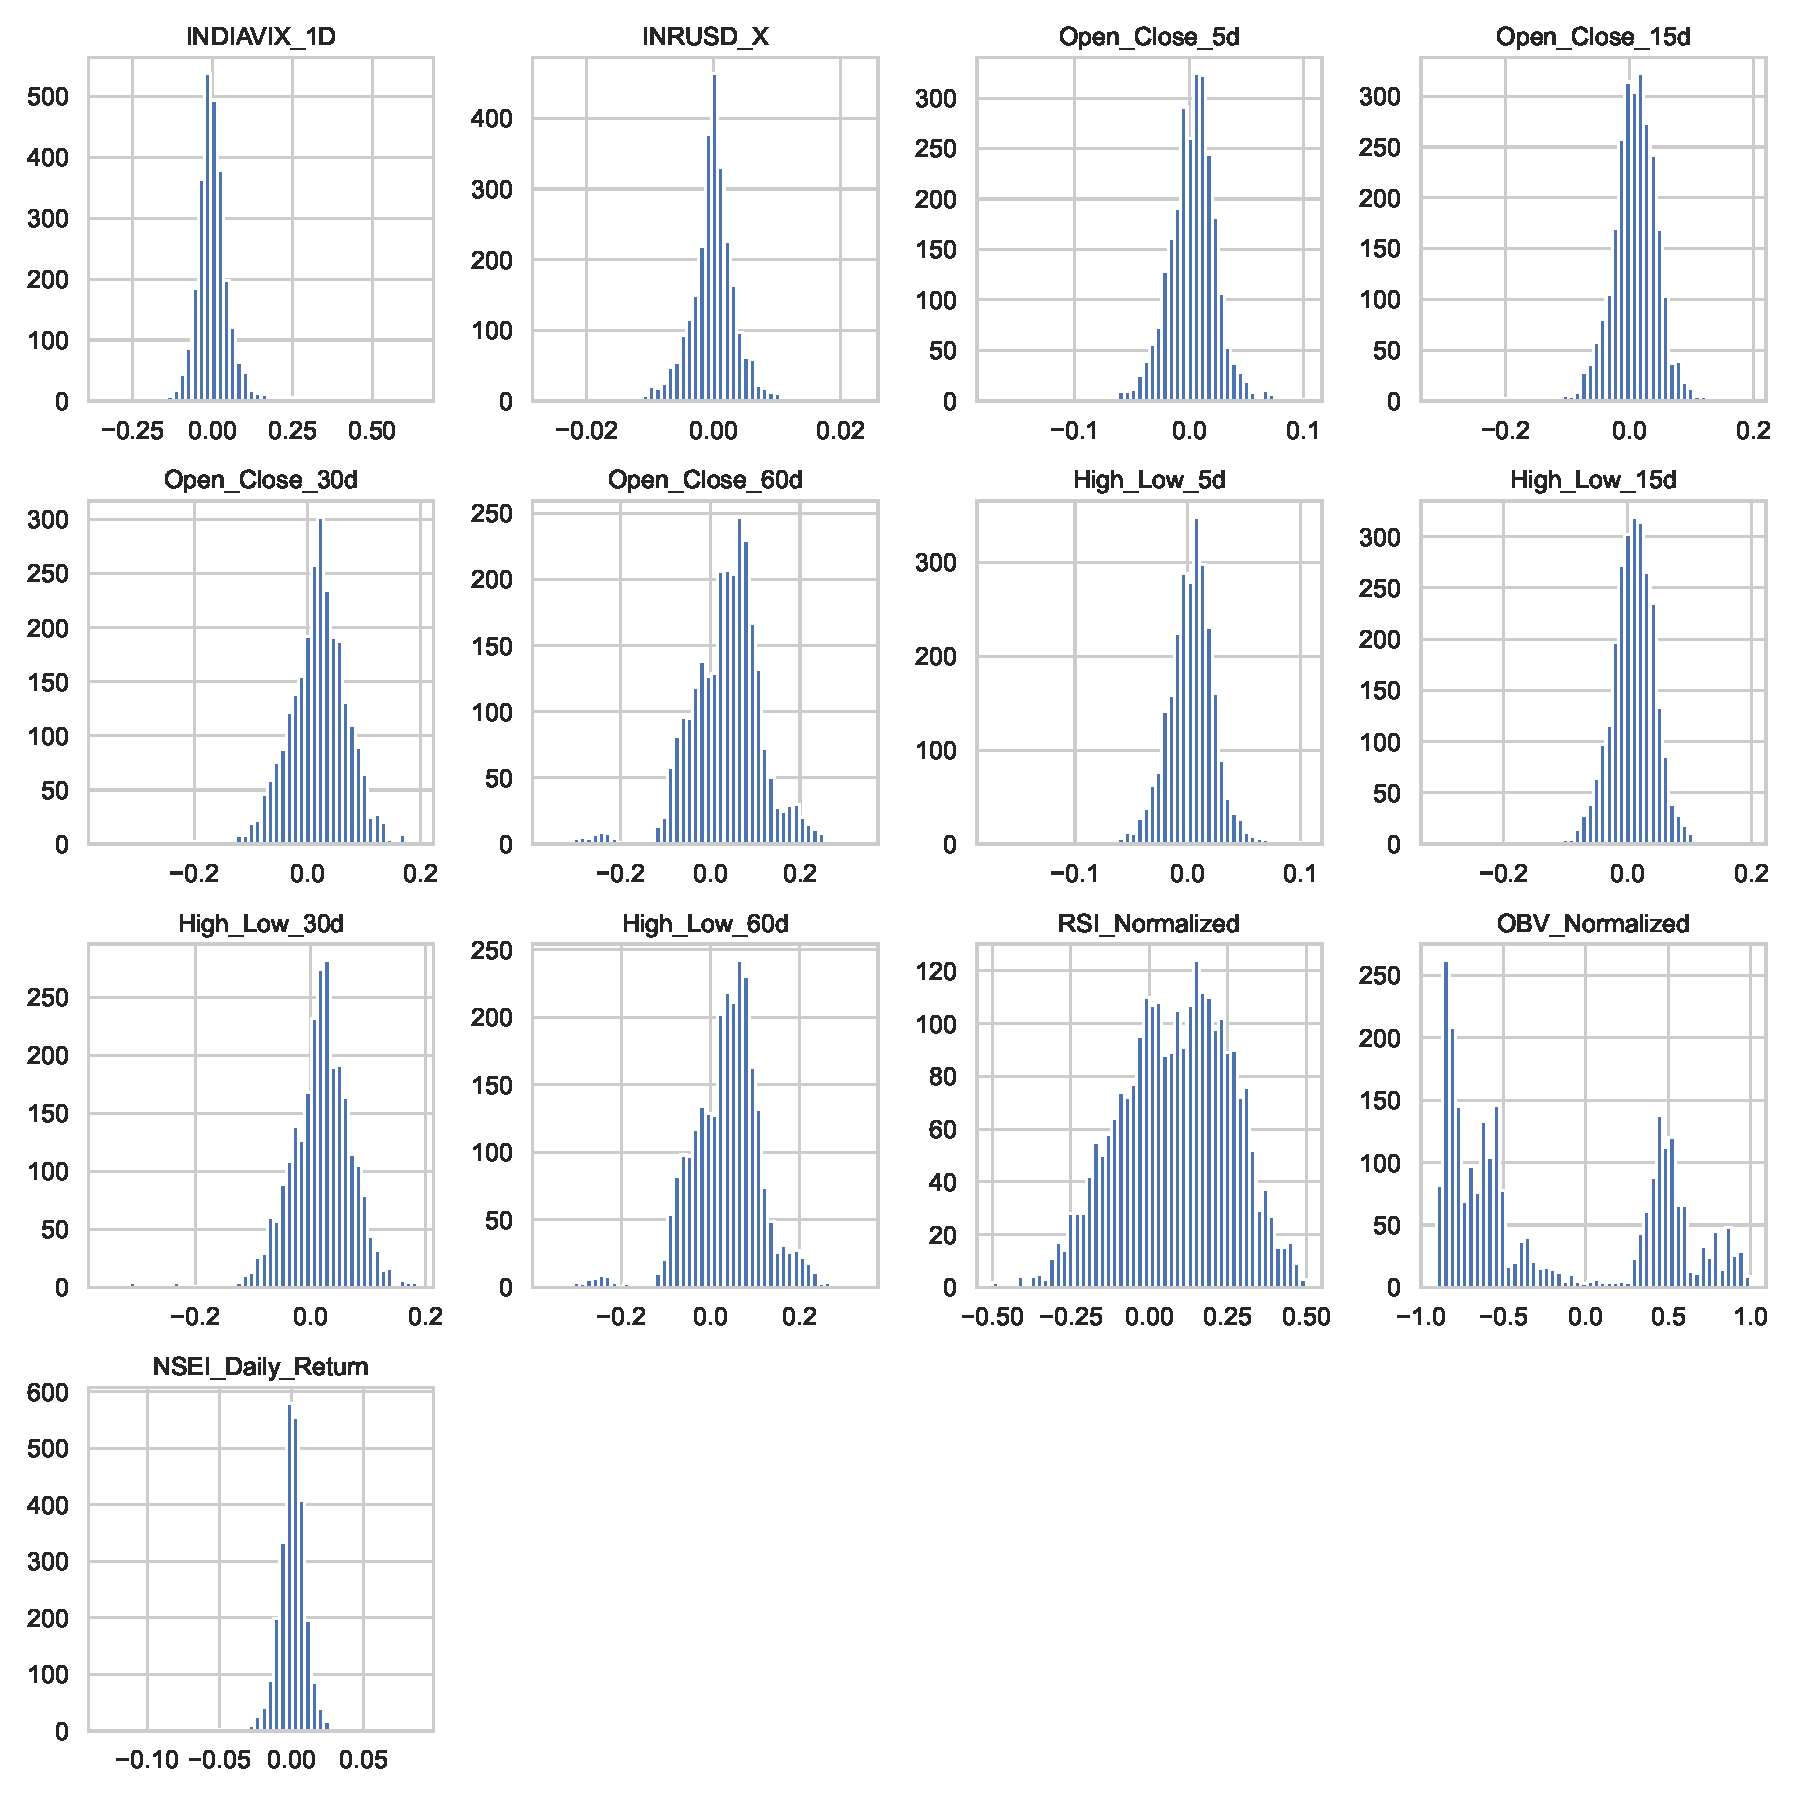
\includegraphics[width=\textwidth]{Images/feature_distributions.pdf}
    \caption{Distribution plots of all features used in the forecasting framework.}
    \label{fig:feature_distributions}
\end{figure}

Additionally, the correlation matrix for all features is displayed in Figure~\ref{fig:correlation_plot}. This plot provides insights into feature interdependencies and the strength of their relationships with the target variable.

\begin{figure}[h!]
    \centering
    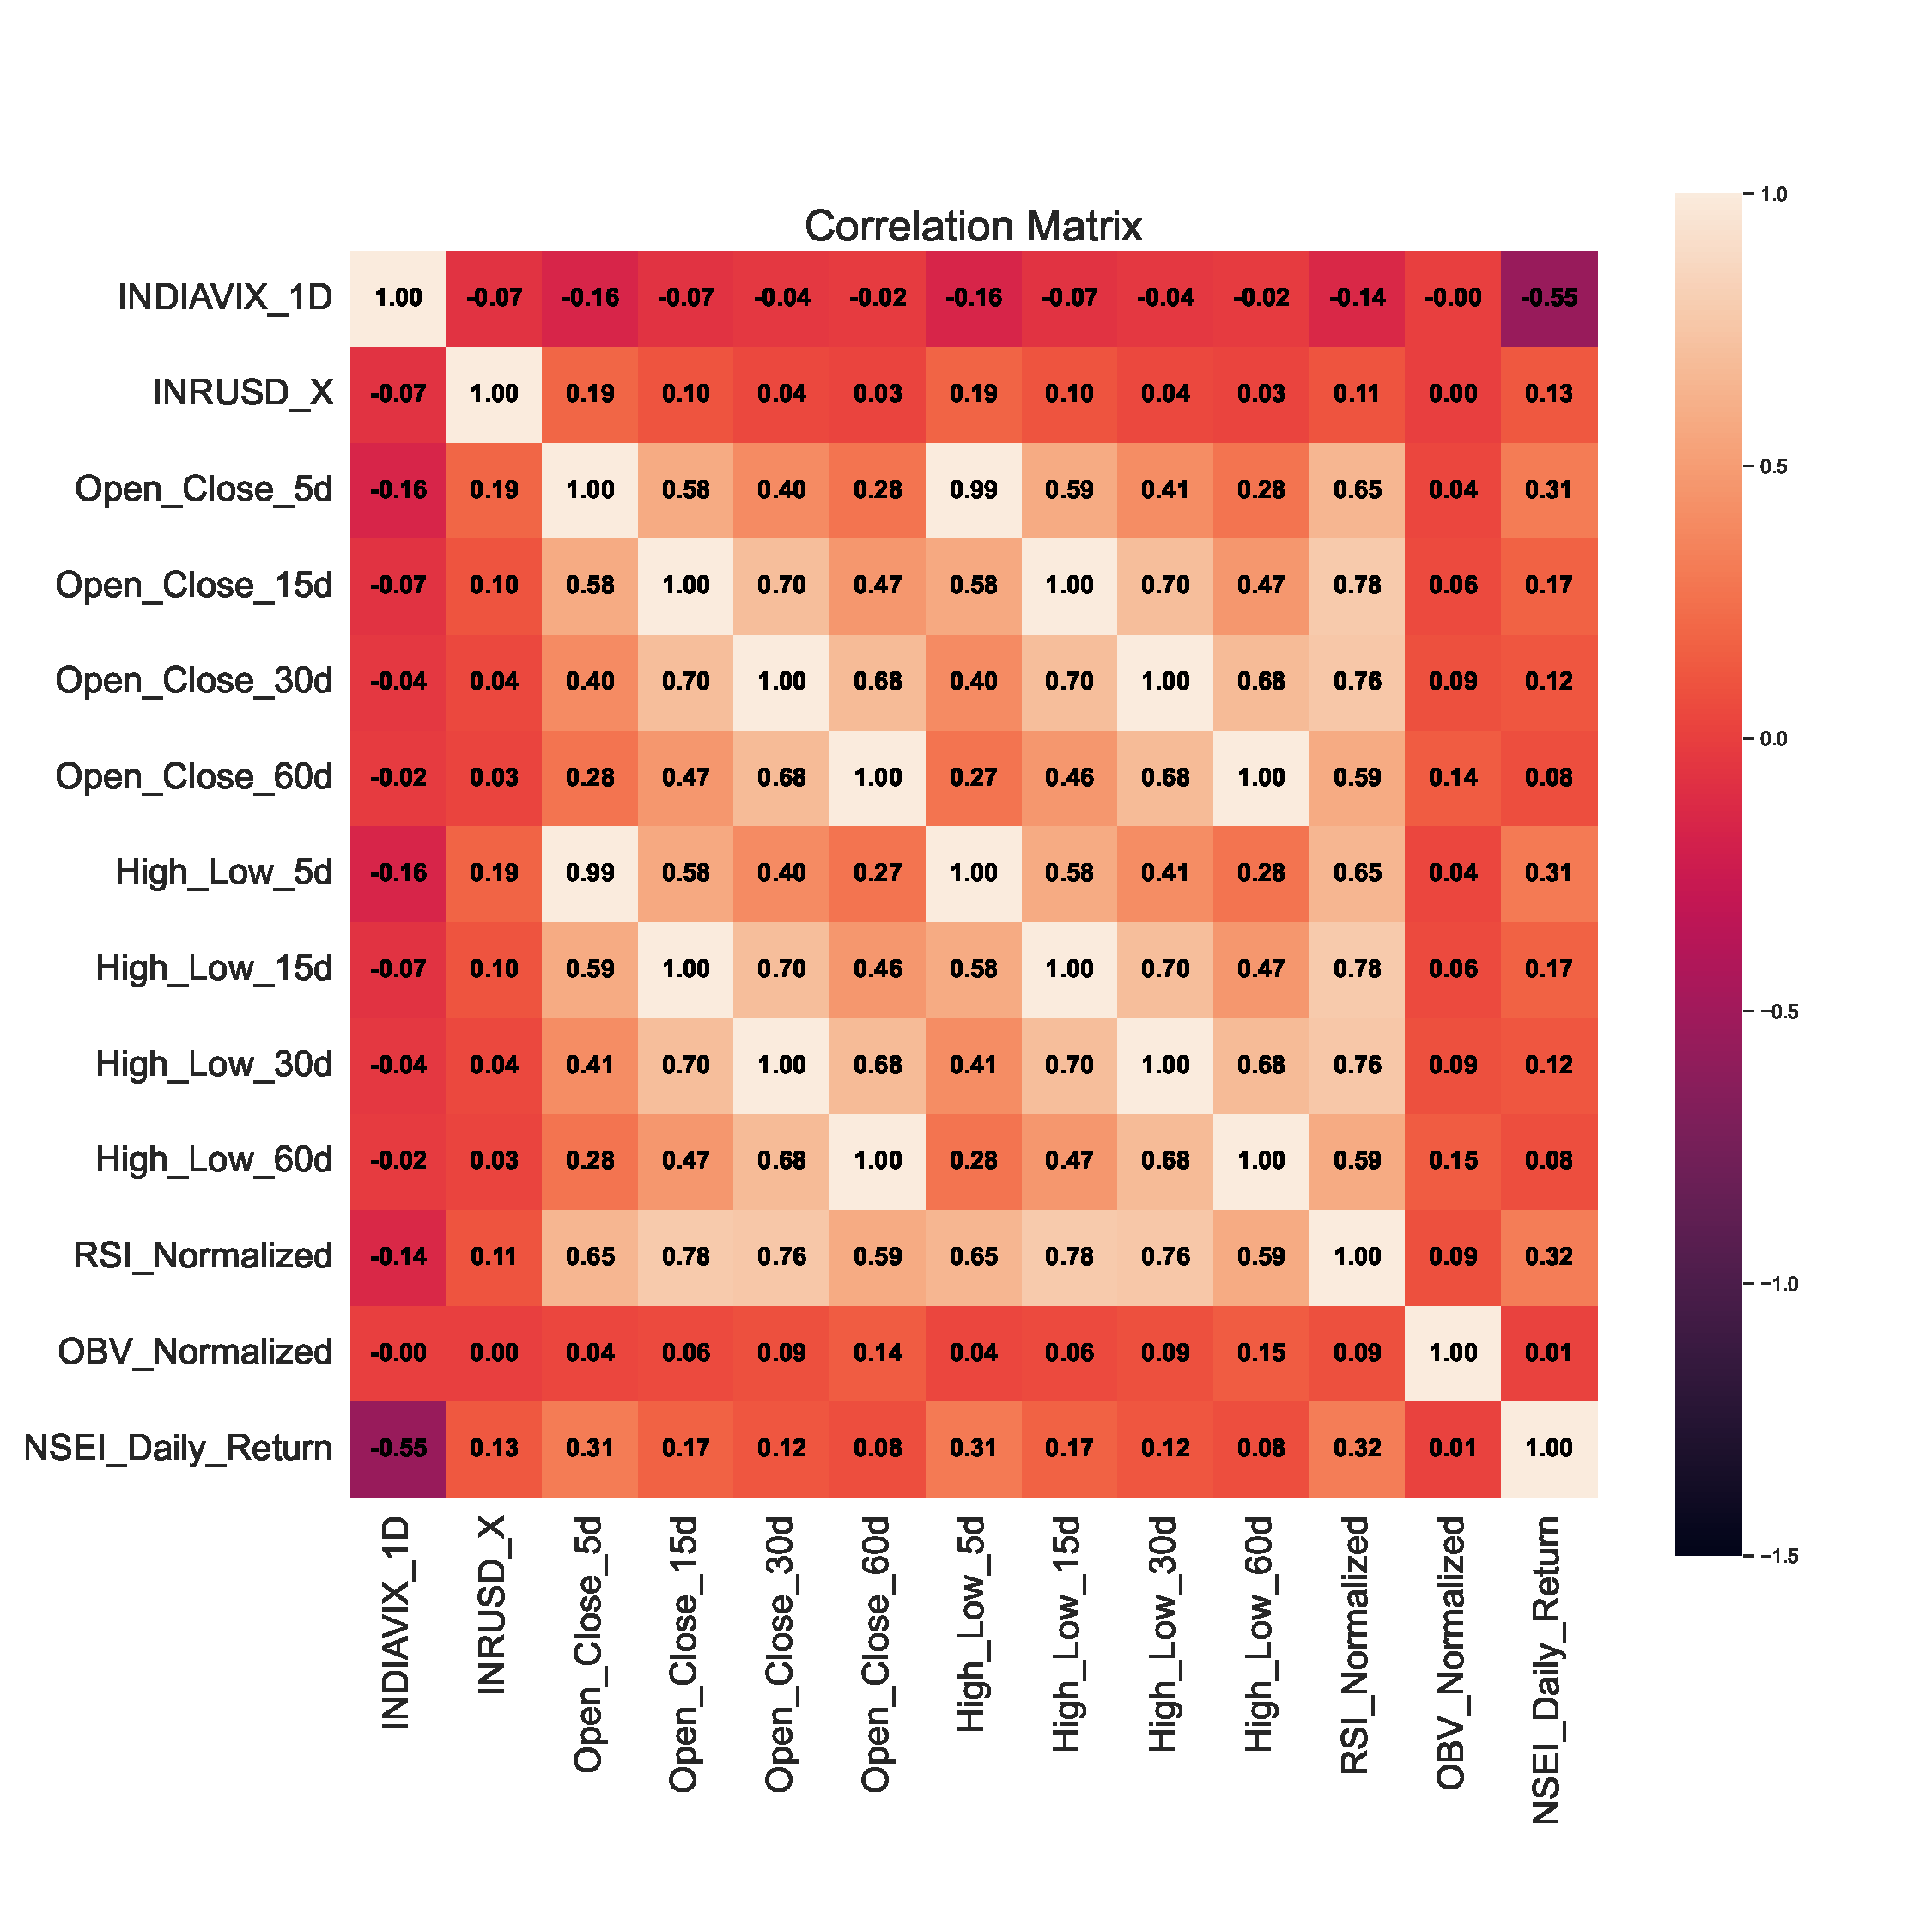
\includegraphics[width=\textwidth]{Images/correlation_plot.pdf}
    \caption{Correlation matrix of all features in the dataset.}
    \label{fig:correlation_plot}
\end{figure}

Finally, Figure~\ref{fig:seasonal_decomposition} presents the seasonal decomposition plot of NSEI close values, illustrating the observed trend, seasonality, and residual components. This visualization assists in understanding the underlying temporal patterns of the target variable.

\begin{figure}[h!]
    \centering
    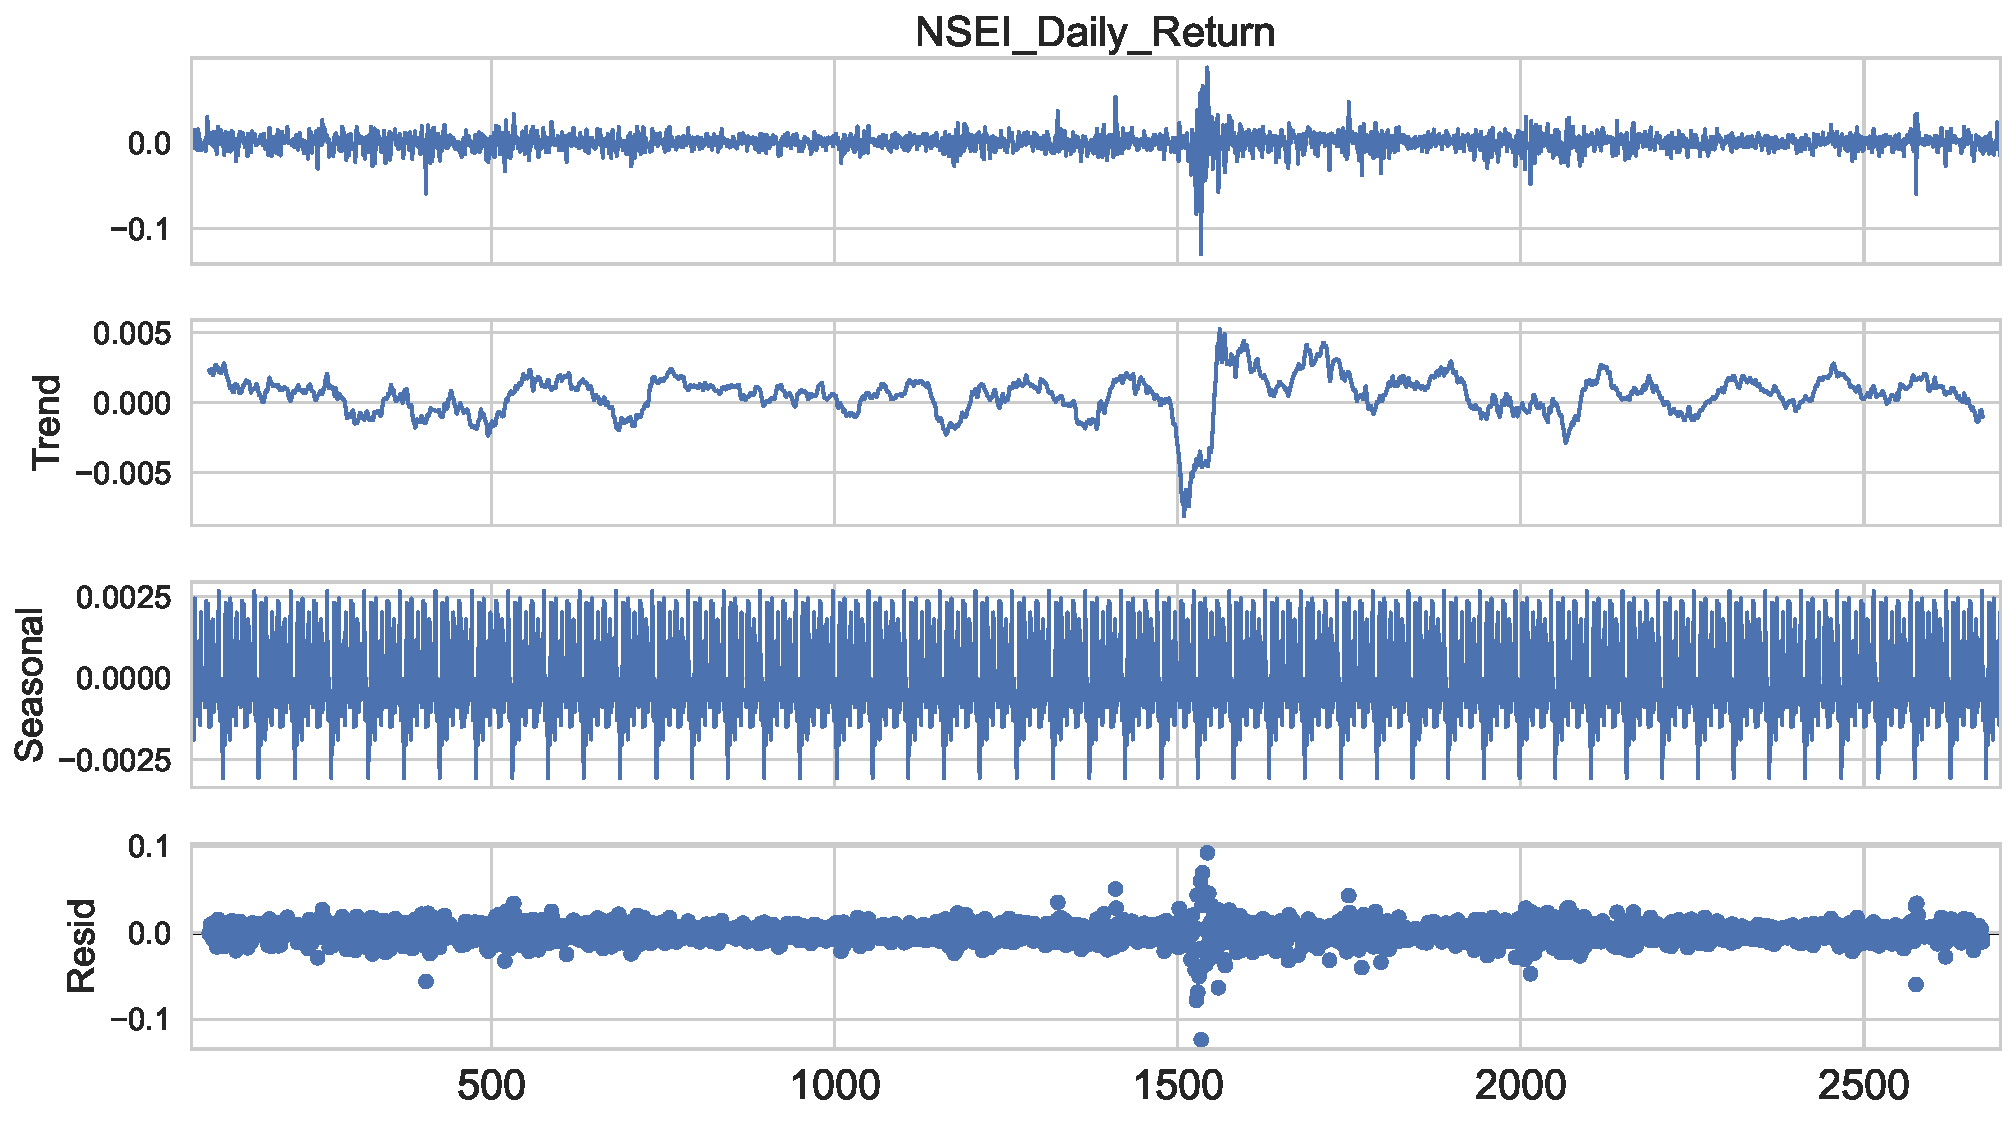
\includegraphics[width=\textwidth]{Images/seasonal_decomposition.pdf}
    \caption{Seasonal decomposition of NSEI close values.}
    \label{fig:seasonal_decomposition}
\end{figure}

\subsection{Feature Selection Using SelectKBest}
Feature selection was performed using the SelectKBest method with \texttt{f\_regression}. The feature importance scores are presented in Table~\ref{tab:feature_importance}.

\begin{table}[h!]
\centering
\caption{Feature Importance Scores using SelectKBest}
\begin{tabular}{|l|c|}
\hline
\textbf{Feature} & \textbf{Score} \\ \hline
INDIAVIX\_1D     & 1125.250181    \\ \hline
RSI\_Normalized  & 292.775295     \\ \hline
Open\_Close\_5d  & 276.984547     \\ \hline
High\_Low\_5d    & 268.947328     \\ \hline
High\_Low\_15d   & 79.876745      \\ \hline
Open\_Close\_15d & 79.634278      \\ \hline
INRUSD\_X        & 42.357608      \\ \hline
Open\_Close\_30d & 35.719346      \\ \hline
High\_Low\_30d   & 35.259659      \\ \hline
Open\_Close\_60d & 16.824506      \\ \hline
High\_Low\_60d   & 16.235917      \\ \hline
OBV\_Normalized  & 0.570088       \\ \hline
\end{tabular}

\label{tab:feature_importance}
\end{table}

\subsection{Feature Refinement}
Low-importance features such as OBV\_Normalized and 30-day/60-day returns were dropped. The refined feature set ensured better model performance with reduced complexity.

\section{GARCH for Stock Price Prediction}

\subsection{Introduction to GARCH}

The Generalized Autoregressive Conditional Heteroskedasticity (GARCH) model is widely used in financial time series modeling due to its ability to capture volatility clustering. In stock markets, volatility tends to persist over time, meaning that periods of high volatility are often followed by more volatile periods, and similarly for low volatility. Since the target variable in this study is \textbf{daily returns}, which inherently exhibits volatility characteristics, GARCH is a suitable choice for modeling this behavior.

GARCH is particularly relevant to this study because it models conditional variance, providing insights into future uncertainty levels. By leveraging GARCH, we aim to enhance stock return prediction by explicitly modeling the variance dynamics, which traditional models might overlook.

\subsection{Model Implementation}

To implement GARCH, the following approach was used:

\begin{itemize}
    \item \textbf{Mean Prediction using ARIMAX:} Before applying GARCH, the mean component of stock returns was modeled using the ARIMAX model. ARIMAX extends ARIMA by incorporating external regressors, making it suitable for capturing linear dependencies in stock returns.
    \item \textbf{Residuals Extraction:} After obtaining the ARIMAX predictions, the residuals (unexplained variations) were extracted. These residuals capture the unpredictable fluctuations in returns.
    \item \textbf{GARCH Modeling on Residuals:} The extracted residuals were then used to train a GARCH model, which estimated the conditional variance of the returns. The GARCH model accounted for volatility clustering, ensuring that periods of high variance were correctly modeled.
\end{itemize}

\subsection{Integration with Existing Architectures}

The GARCH model was not used in isolation but was integrated into the broader framework of stock price prediction. Specifically:

\begin{itemize}
    \item The \textbf{ARIMAX model} was used for predicting the mean returns.
    \item The \textbf{GARCH model} was applied to the residuals from ARIMAX to model volatility.
    \item The final output was a combination of the ARIMAX-predicted mean and the variance estimation from the GARCH model, providing a more comprehensive prediction of stock returns.
\end{itemize}

By integrating GARCH with ARIMAX, the model was able to separately handle both the trend and volatility components of stock returns, improving the overall robustness of the forecasting framework.



% \chapter{Frameworks and Models for Stock Price Prediction}

% \section{Overview of Proposed Architectures}
% This chapter provides a detailed explanation of various architectures designed and developed for stock price prediction. Starting from the Hybrid LSTM-RLS Architecture created during the summer internship, subsequent modifications and alternative models are described, highlighting their strengths, limitations, and outcomes.

% \section{Hybrid LSTM-RLS Architecture}

% \subsection{Workflow and Design}

% The Hybrid LSTM-RLS architecture was developed during my summer internship. It combines the strengths of Long Short-Term Memory (LSTM) networks for sequential data modeling with Recursive Least Squares (RLS) for refining predictions.

% \begin{figure}[h!]
%     \centering
%     \includegraphics[width=0.8\textwidth]{SummerInternArchitecture.pdf} % Adjust width as needed
%     \caption{Hybrid LSTM-RLS Architecture}
% \label{fig:summerarch}
% \end{figure}

% Figure \ref{fig:summerarch} illustrates the workflow of this architecture. Key steps are as follows:
% \begin{enumerate}
%     \item \textbf{Install and load necessary libraries:} 
%     \begin{itemize}
%         \item Libraries such as tensorflow, numpy, yfinance and scikit- learn are installed and imported.
%     \end{itemize}
    
%     \item \textbf{Load stock data using yfinance API:} 
%     \begin{itemize}
%         \item Data representing price of the stocks in any given time is extracted from yfinance API for the desired time.
%     \end{itemize}
    
%     \item \textbf{Data preprocessing:} 
%     \begin{itemize}
%         \item Preprocessing of data is also performed, which consists of normalization, missing values dealt and the splitting of data in training and testing.
%     \end{itemize}
    
%     \item \textbf{Create sequences:}
%     \begin{itemize}
%         \item Price sequences of stocks are generated for making the data ready for LSTM
% model. Every one of these sequences includes information about the past price level for training purposes.
%     \end{itemize}
    
%     \item \textbf{Train the LSTM model:}
%     \begin{itemize}
%         \item Using these sequences, LSTM model is prepared and tested for predicting the next value of the stock.
%     \end{itemize}
    
%     \item \textbf{LSTM predictions passed to RLS model:}
%     \begin{itemize}
%         \item The scalar predictions from the LSTM model are taken as an input by the RLS algorithm.
%     \end{itemize}
    
%     \item \textbf{RLS model provides final prediction:}
%     \begin{itemize}
%         \item The RLS model processes the LSTM prediction and from it produces the final stock price prediction.
%     \end{itemize}
    
% \end{enumerate}

% \section{Enhanced Hybrid LSTM-RLS Architecture}

% To address issues such as dimension mismatches and long training times in the original architecture, several enhancements were implemented in Semester 3. These refinements simplified the process and improved predictive accuracy.

% Figure \ref{fig:Refinedarch} illustrates the improved workflow:

% After I started Semester 3, I improved the architecture developed in this early figure \ref{fig:Refinedarch}. Such improvements were executed to make the architecture more predictable and to solve problems such as dimension mismatch and long training times. It made the model much simpler and highly efficient to use for stock price forecasting.

% \subsection{Architecture Workflow}

% \begin{figure}[htbp]
%     \centering
%     \includegraphics[width=0.8\textwidth]{RefinedArchitecture.pdf} % Adjust width as needed
%     \caption{Enhanced Hybrid LSTM-RLS Architecture}
% \label{fig:Refinedarch}
% \end{figure}

% Architecture process involves the following steps:

% \begin{enumerate}
%     \item \textbf{Install and import necessary libraries:}
%     \begin{itemize}
%         \item All libraries are imported as like yfinance, tensorflow, scikit-learn and so on.
%     \end{itemize}
    
%     \item \textbf{Import Nifty 50 daily close price data:}
%     \begin{itemize}
%         \item For the last 12 years, it fetches the closing prices of Nifty 50 from the yfinance API daily.
%     \end{itemize}
    
%     \item \textbf{Normalize the data:}
%     \begin{itemize}
%         \item Normalized the data and scaled it between 0 to 1 and fed it into the LSTM model. This was done using MinMaxScaler.
%     \end{itemize}
    
%     \item \textbf{Create sequences for LSTM:}
%     \begin{itemize}
%         \item Sequences of past stock prices are created to prepare the data for LSTM training.
%     \end{itemize}
    
%     \item \textbf{Divide the data into 80\% training and 20\% testing:}
%     \begin{itemize}
%         \item The sequences are divided into 80\% for training and 20\% for testing.
%     \end{itemize}
    
%     \item \textbf{Train the LSTM model:}
%     \begin{itemize}
%         \item The LSTM model is trained on the 80\% training data over several epochs to predict the stock prices.
%     \end{itemize}
    
%     \item \textbf{Use LSTM to forecast:}
%     \begin{itemize}
%         \item The trained LSTM model provides predictions for both the train and test sets.
%     \end{itemize}
    
%     \item \textbf{Sequences used in RLS model input:}
%     \begin{itemize}
%         \item The LSTM model predictions are used to create input sequences for the Recursive Least Squares (RLS) model.
%     \end{itemize}
    
%     \item \textbf{Forecast final stock prices using the RLS model:}
%     \begin{itemize}
%         \item The RLS model uses the LSTM predictions as input and outputs the final stock price predictions.
%     \end{itemize}
    
% \end{enumerate}

% \subsection{Developing Input Sequences for RLS}

% \begin{figure}[htbp]
%     \centering
%     \includegraphics[width=0.8\textwidth]{RLSInputCreation.pdf} % Adjust width as needed
%     \caption{Input Sequence Formation}
% \label{fig:inputseq}
% \end{figure}

% The following steps are followed to generate the input sequences for the RLS model based on LSTM predictions:

% \begin{enumerate}
%     \item \textbf{Original Sequence for LSTM:} 
%     \begin{itemize}
%         \item The original sequence of stock prices is used as the input to the LSTM model. 
%         \item For example, a sequence from index 0 to 49 is selected.
%     \end{itemize}

%     \item \textbf{Training the LSTM Model:}
%     \begin{itemize}
%         \item The LSTM model is trained on the input sequence.
%         \item After training, the LSTM model generates a prediction, i.e., the 50th value based on the past 49 values.
%     \end{itemize}

%     \item \textbf{Shifting the Sequence for RLS Input:}
%     \begin{itemize}
%         \item The sequence used for LSTM training is shifted by one step to create the input for the RLS model.
%         \item For instance, the sequence now starts from index 1 and runs up to index 50.
%         \item The prediction generated by the trained LSTM model for the 50th point is appended to this new sequence.
%     \end{itemize}

%     \item \textbf{Final Input for RLS Model:}
%     \begin{itemize}
%         \item The shifted sequence (from 1 to 50) is provided as input to the RLS model.
%         \item The RLS model uses this input to generate the final stock price prediction.
%     \end{itemize}
% \end{enumerate}

% This process enables the integration of the LSTM predictions with the RLS model by using a sequential sliding window approach.

% \section{Dual Network Solution Architecture}
% The RMSE and R\(^2\) score of the Enhanced Hybrid LSTM-RLS architecture show good performance, but there exists a constant lag of 1 time step in the predictions. This results in a relatively higher RMSE error of 0.76\%. To address this lag, I adopted the Dual Network Solution (DNS) architecture proposed by \textcite{samanta_dual_2020}, which is designed to reduce such time-step lags in forecasting.

% Figure \ref{fig:DNSArch} illustrates the architecture of the Dual Network Solution (DNS) Architecture, which operates as follows:

% \begin{enumerate}
%     \item \textbf{Training Network 1}: 
%     Network 1 is trained on trends extracted from actual data using the Slope Difference Method or Moving Averages.
    
%     \item \textbf{Training Network 2}: 
%     Network 2 is trained directly on the actual data.
    
%     \item \textbf{Lag-Free Prediction}: 
%     After training, the models are used for lag-free predictions.
    
%     \item \textbf{Input to Network 1}: 
%     The actual data is passed as input to Network 1, which predicts the trend based on this input.
    
%     \item \textbf{Input to Network 2}: 
%     The predicted trend from Network 1 is then provided as input to Network 2 to obtain the final prediction.
% \end{enumerate}

% \begin{figure}[htbp]
%     \centering
%     \includegraphics[width=0.8\textwidth]{23MAI004_Sem3_MidSem_Report/DNSArchitecture.pdf} % Adjust width as needed
%     \caption{DNS Architecture}
% \label{fig:DNSArch}
% \end{figure}

% \section{ARIMA-LSTM Residual Integration Framework}

% In this section, I have employed a hybrid model aimed at addressing the lag observed in the results of the Dual Network Solution (DNS) architecture discussed previously. The model architecture used here is inspired by the framework proposed by Shah et al. In their approach, the authors decompose the final stock price prediction into three components: \textbf{linear}, \textbf{non-linear}, and \textbf{error}.

% \begin{itemize}
%     \item \textbf{Linear Component}: The ARIMA model is employed to make an initial prediction by capturing the linear component in the data. The residuals are then computed as the difference between the actual values and the ARIMA predictions.  
%     \item \textbf{Non-linear Component}: The calculated residuals are used as input to an LSTM model, which is trained to capture the non-linear component of the data.  
%     \item \textbf{Final Prediction}: The predictions from the ARIMA model and the LSTM model are combined to obtain the final stock price predictions.
% \end{itemize}

% To build upon this framework, I have made modifications by employing the LSTM model to predict both the linear and non-linear components of the data. This adjustment aims to enhance the model’s flexibility and predictive accuracy. The complete flow of the proposed architecture, including its modifications, is illustrated in \textbf{Figure 1}.

% \section{Multi-Feature LSTM Forecasting Framework}

% As the \textbf{ARIMA-LSTM Residual Integration Framework} was unable to effectively remove the lag in predictions and its performance degraded compared to other proposed models, I decided to adopt a \textbf{Multi-Feature LSTM Forecasting Framework}. This approach utilizes multiple features as input to train the LSTM architecture, aiming to improve the predictive accuracy and eliminate lag.

% \subsection{Feature Engineering}

% The dataset includes the following features:
% \begin{itemize}
%     \item \textbf{5-day, 15-day, 30-day, and 60-day returns} calculated using the average of high and low values of NSEI.
%     \item \textbf{5-day, 15-day, 30-day, and 60-day returns} calculated using the average of open and close values of NSEI.
%     \item \textbf{RSI (Relative Strength Index)} values calculated on daily close values, normalized to a range of \([-0.5, 0.5]\).
%     \item \textbf{OBV (On-Balance Volume)} values calculated using close values and volume of NSEI, normalized to a range of \([-1, 1]\).
%     \item \textbf{1-day returns} calculated on daily close values of INR-USD currency exchange data.
%     \item \textbf{1-day returns} calculated on daily close values of the \(^\text{INDIAVIX}\) index.
% \end{itemize}

% All return values were kept in their original scale, while RSI and OBV were normalized for consistency.

% The entire dataset is visualized using histograms, correlation plots, and pair plots, which are shown below.


% \subsection{Feature Selection Using SelectKBest}

% To refine the dataset, I applied the \textbf{SelectKBest} feature selection method with \texttt{f\_regression} as the scoring function. The input features were evaluated against the daily returns calculated on daily close values of NSEI as the output. The importance scores of the features are presented in Table~\ref{tab:feature_importance}.

% \begin{table}[H]
% \centering
% \begin{tabular}{|l|c|}
% \hline
% \textbf{Feature} & \textbf{Score} \\ \hline
% INDIAVIX\_1D     & 1125.250181    \\ \hline
% RSI\_Normalized  & 292.775295     \\ \hline
% Open\_Close\_5d  & 276.984547     \\ \hline
% High\_Low\_5d    & 268.947328     \\ \hline
% High\_Low\_15d   & 79.876745      \\ \hline
% Open\_Close\_15d & 79.634278      \\ \hline
% INRUSD\_X        & 42.357608      \\ \hline
% Open\_Close\_30d & 35.719346      \\ \hline
% High\_Low\_30d   & 35.259659      \\ \hline
% Open\_Close\_60d & 16.824506      \\ \hline
% High\_Low\_60d   & 16.235917      \\ \hline
% OBV\_Normalized  & 0.570088       \\ \hline
% % Unnamed: 0       & 0.075218       \\ \hline
% \end{tabular}
% \caption{Feature Importance Scores using SelectKBest}
% \label{tab:feature_importance}
% \end{table}

% \subsection{Feature Refinement}

% Based on the feature importance scores, the following features were dropped due to their low relevance:
% \begin{itemize}
%     \item \textbf{OBV\_Normalized}: Score of 0.570088.
%     \item \textbf{30-day and 60-day returns} calculated for both \textbf{open-close} and \textbf{high-low} averages.
% \end{itemize}

% The refined feature set focuses on the most important predictors, ensuring improved model performance while reducing complexity.